\documentclass[margin=2mm]{standalone}

\usepackage{tikz}
\usetikzlibrary{positioning,calc}

\begin{document}
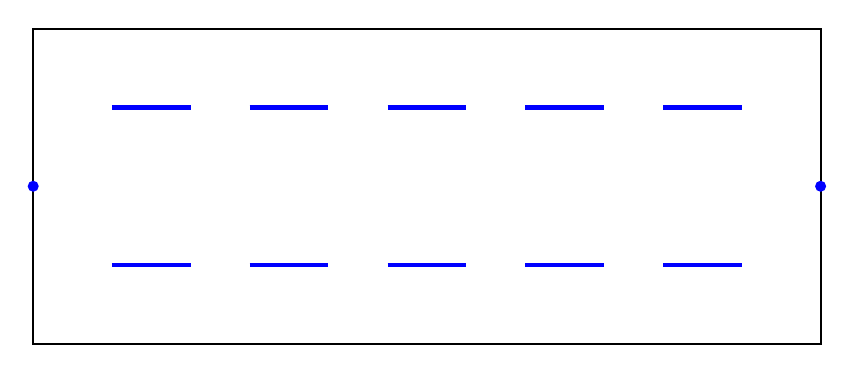
\begin{tikzpicture}
    \draw[thick] (0,0) rectangle ++(10,4);


    \foreach \x in {0,1,2,3,4} {
        \draw[ultra thick,blue] (1.75*\x+1,1) -- ++(1,0);
    }
    \foreach \x in {0,1,2,3,4} {
        \draw[ultra thick,blue] (1.75*\x+1,3) -- ++(1,0);
    }

    \fill[blue] (0,2) circle(2pt);
    \fill[blue] (10,2) circle(2pt);

\end{tikzpicture}
\end{document}